% Chapter 13

\chapter{Análisis de Resultados} % Write in your own chapter title
\label{Chapter13}
\lhead{Capítulo 13. \emph{Resultados}} % Write in your own chapter title to set the page header

En este capítulo se muestran los resultados obtenidos en la implementación del hardware. Para esto se siguió la metodología descrita en el capítulo \ref{Chapter11}: 
 
 \section{Benchmark}
Dada la necesidad de medir el rendimiento del circuito implementado en HW contra la versión SW, se determinó que la mejor métrica se obtendría realizando un Benchmark de tres etapas con ejecuciones de 100 (\textbf{SW\_ 100M}) y 300 millones de operaciones por ejecución (\textbf{SW\_ 300M}), con la implementación en HW funcionando a 100MHz (\textbf{HW\_ 100M\_ 100MHz}, \textbf{HW\_ 300M\_ 100MHz}) y 150MHz (\textbf{HW\_ 100M\_ 150MHz}, \textbf{HW\_ 300M\_ 150MHz}), que son las frecuencias de reloj recomendadas por el sintetizador de alto nivel. La prueba consiste en cargar las neuronas de entrada y calcular el tiempo que le tomó a ambas aproximaciones realizar el cálculo del resultado.

Como se observa en la Figura \ref{fig:benchmark}, las implementaciones \textbf{HW\_ 100M\_ 100MHz}, \textbf{HW\_ 100M\_ 150MHz}, \textbf{HW\_ 300M\_ 100MHz} y \textbf{HW\_ 300M\_ 150MHz} comparado con las implementaciones \textbf{SW\_ 100M} y \textbf{SW\_ 300M} la aceleración es aproximadamente cuatro veces. Esta prueba lo que busca es saturar el bus AMBA cargando y exigiendo al máximo el pipeline del bus usando las optimizaciones burst de la interfaz AXI. A diferencia de la implementación HW, la implementación software realiza una carga de las neuronas de entrada de forma secuencial adicionando un tiempo de carga alto debido a los múltiples llamados al bus que se encarga de la RAM.

%tek Revisar los valores numéricos

 \begin{figure}[!ht]
	\centering
		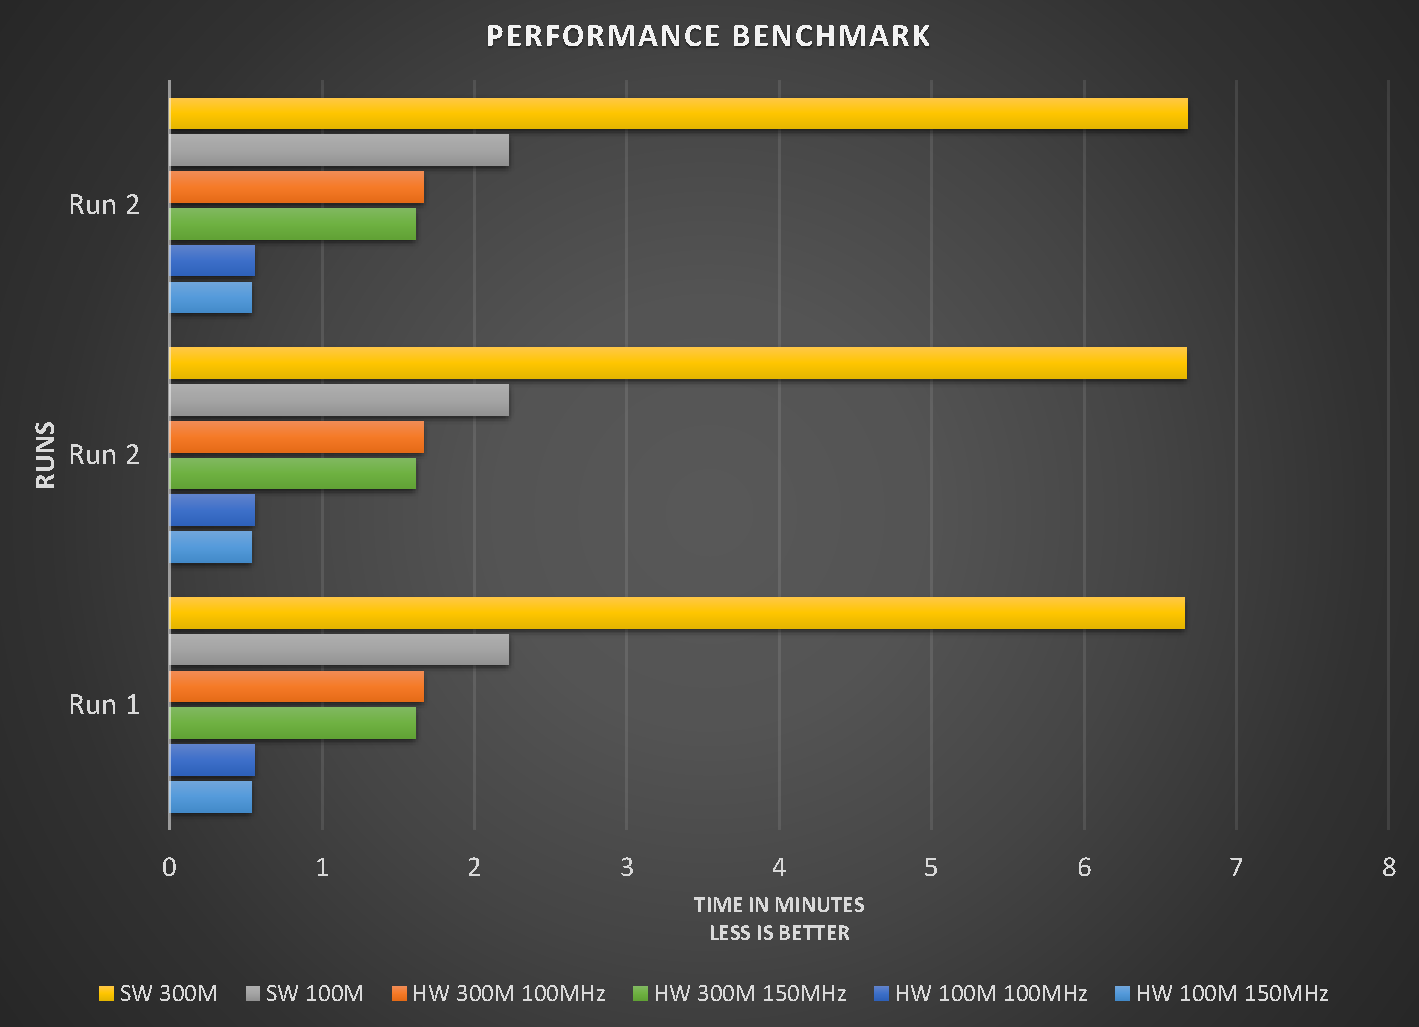
\includegraphics[scale=0.6]{Figures/performanceBenchmark}
	\caption{Benchmark resultados de la implementación}
	\label{fig:benchmark}
\end{figure}


\clearpage

\section{Análisis de tiempo y recursos}
\subsection{Tiempo de ejecución}

En la Figura \ref{fig:generalPerformance} se observan los resultados de la implementación de diferentes estrategias de optimización del hardware; en este caso tenemos: 
\begin{itemize}

\item WO-OPT: Sin optimizaciones.

\item P-UNROLL: Pipelining a nivel de bucles combinado con Unroll a los bucles.

\item DATAFLOW: Pipelining a nivel de tareas.

\item AO: Optimización de área.

\item PO: Pipelining a nivel de tareas, bucles y unroll

\end{itemize}

 \begin{figure}[!ht]
	\centering
		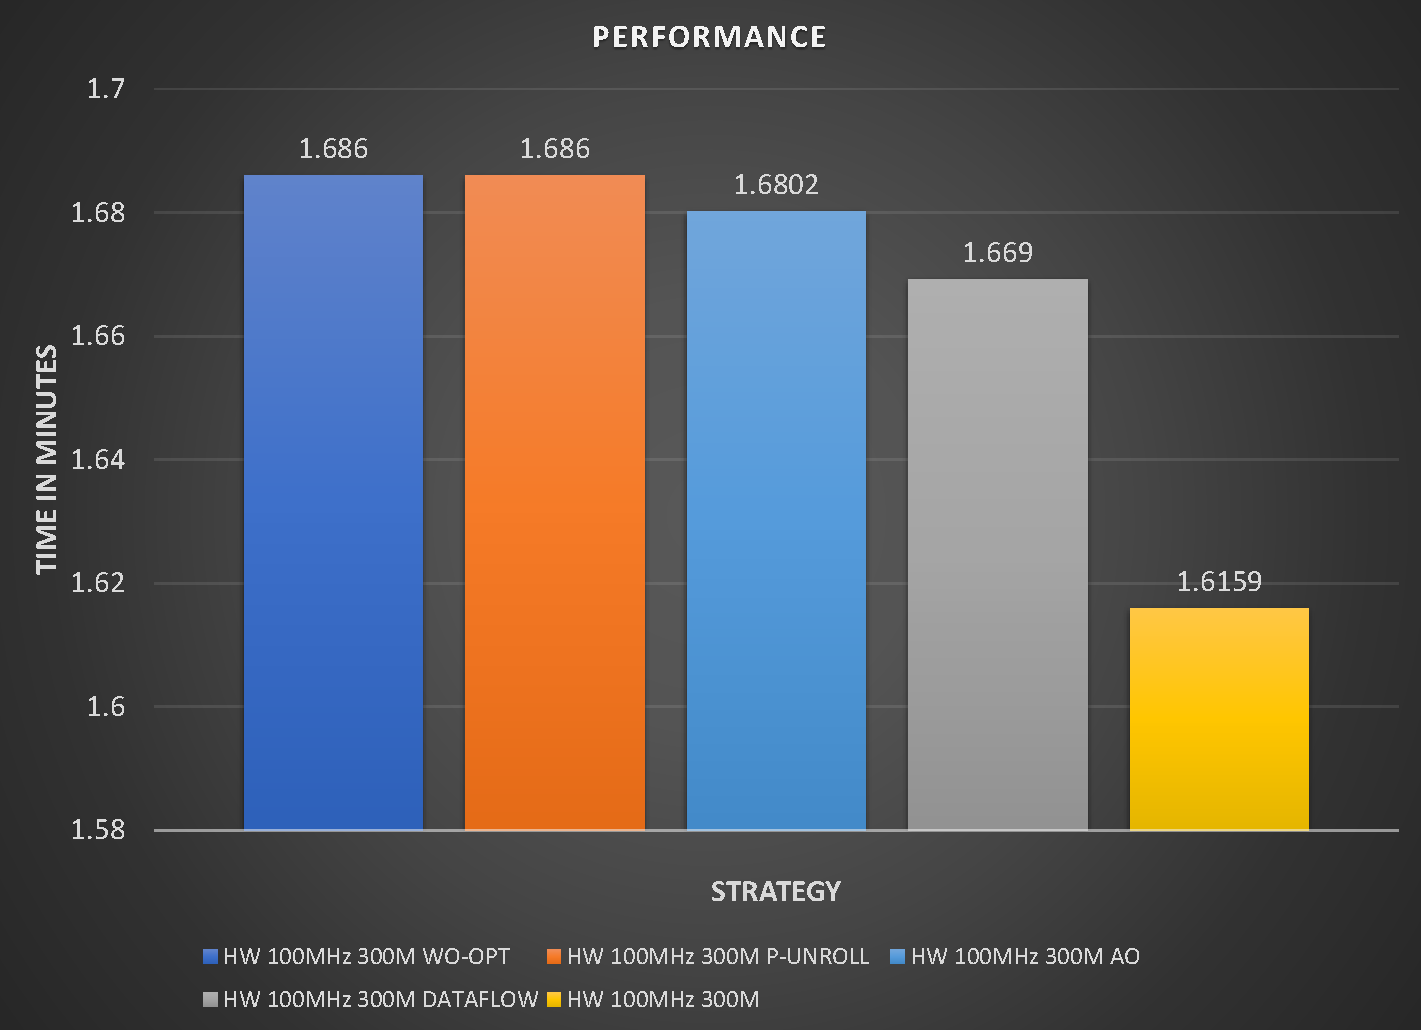
\includegraphics[scale=0.6]{Figures/generalPerformance}
	\caption{Rendimiento del acelerador en Hardware}
	\label{fig:generalPerformance}
\end{figure}

La Figura muestra claramente que la estrategia ``PO'' ofrece el mejor rendimiento en tiempo de ejecución de las tareas, siendo la estrategia a implementar en producción.

\clearpage

\subsection{Recursos utilizados}
Una vez determinados los tiempos de ejecución, se hace necesario tener en cuenta el área o la cantidad de recursos necesarios para cumplir las diferentes tareas de la solución. En este caso se analizó la cantidad de recursos para cada estrategia teniendo en cuenta el reporte del sintetizador de hardware Vivado.

La Figura \ref{fig:usedResources} muestra el porcentaje de recursos usados por cada una de las diferentes estrategias. Es importante notar que la estrategia ``AO'' usa 51\% menos LUT, 42\% menos DSPs y 37\% menos BRAM que su contraparte ``PO'' para un rendimiento casi marginal en tiempo.

\begin{figure}[!ht]
	\centering
		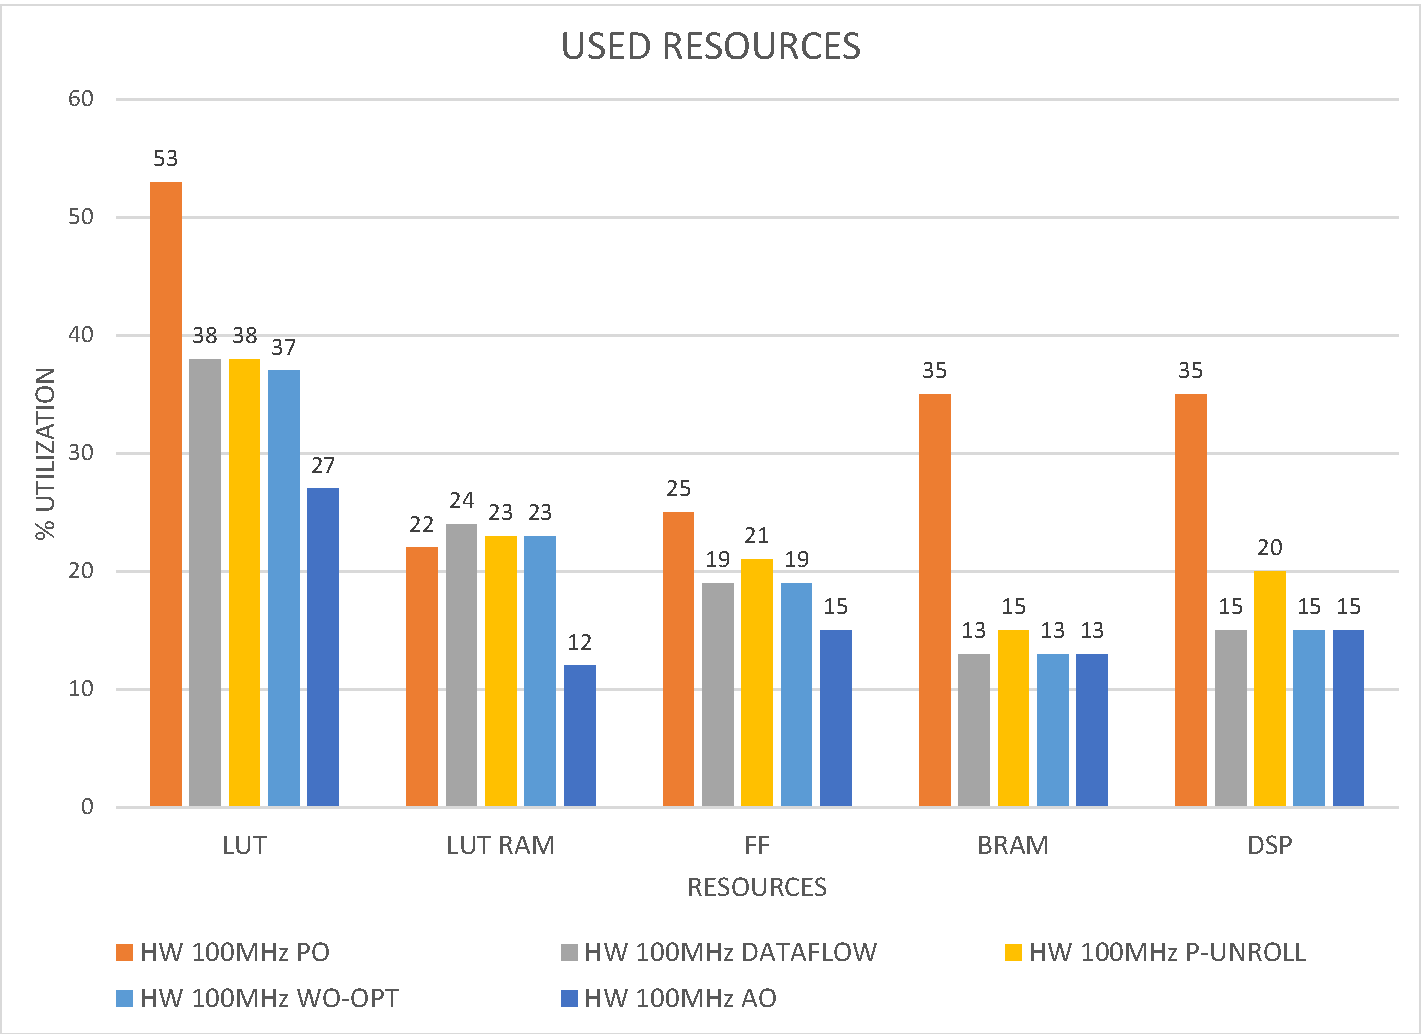
\includegraphics[scale=0.6]{Figures/usedResources}
	\caption{Recursos utilizados en la FPGA}
	\label{fig:usedResources}
\end{figure}

La Figura \ref{fig:performanceResources} muestra claramente que la estrategia ``AO'' es aproximadamente 46\% más eficiente que su contraparte ``PO''. De esta forma, es posible determinar que, al usar menos área vamos a obtener un mejor delta de eficiencia, pues al usar menos recursos es posible adicionar más módulos de hardware o, en otros casos, usar menos potencia en tiempo de ejecución.

\begin{figure}[!ht]
	\centering
		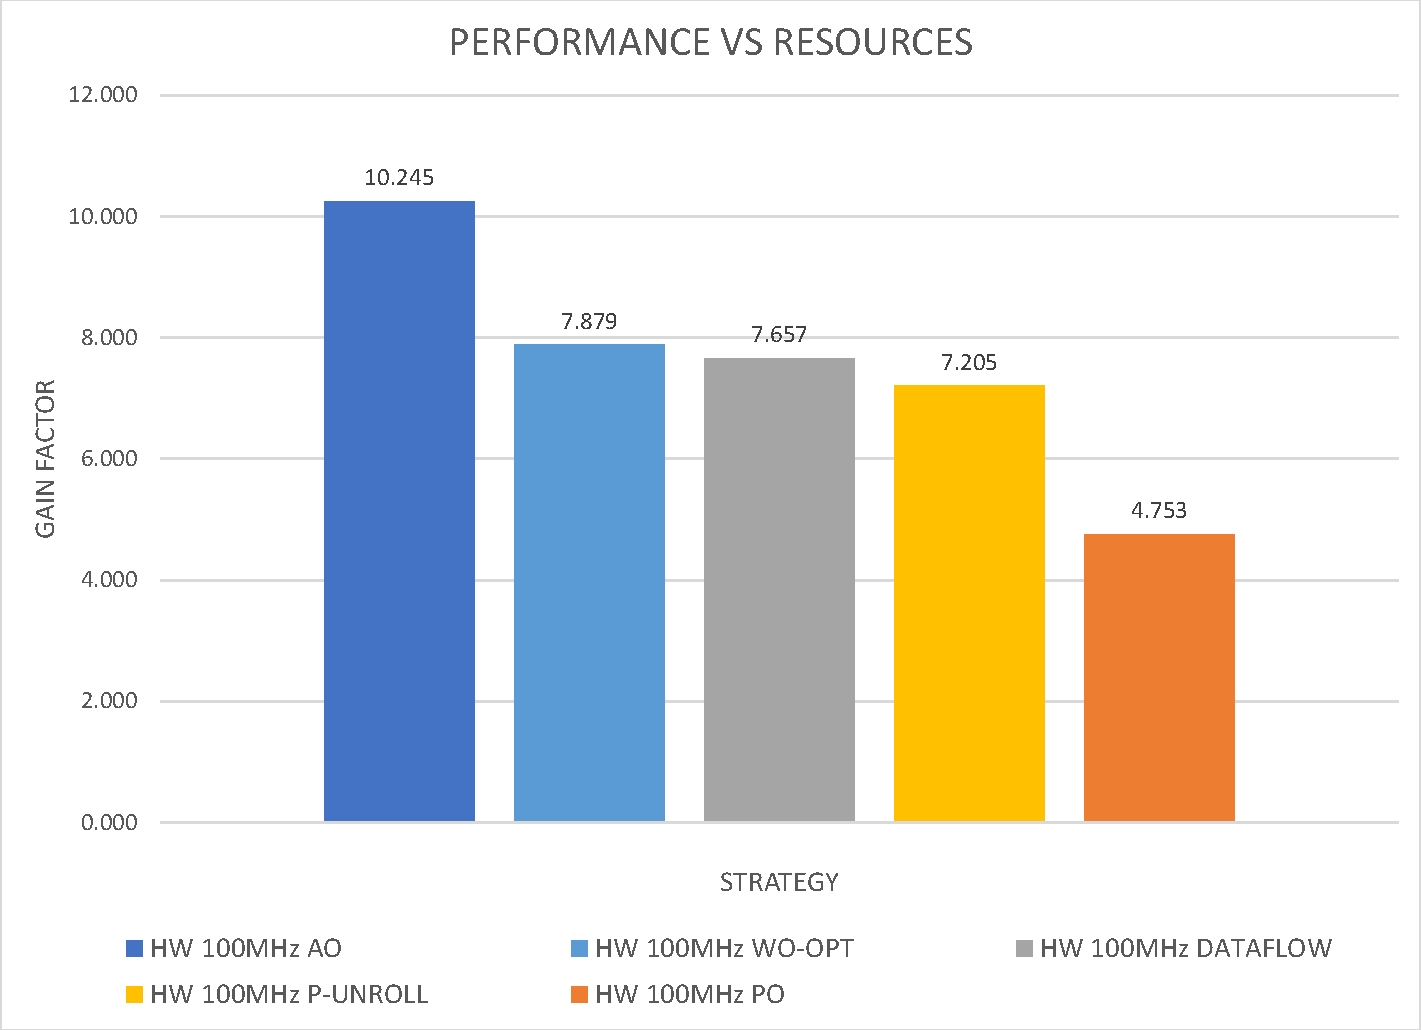
\includegraphics[scale=0.6]{Figures/performanceResources}
	\caption{Factor de ganancia recursos contra tiempo}
	\label{fig:performanceResources}
\end{figure}
